\documentclass[final,3p,times,twocolumn]{elsarticle}

\usepackage{amssymb} %math symbols
\usepackage{graphicx} %[trim]
\usepackage{media9}
\usepackage{enumerate}

\begin{document}

\begin{frontmatter}

\title{Robotics101}

\author{Sergio Azizi}

\begin{abstract}
I built this under the supervision of Chinemelu Ezeh, president of the UCLU Robotics Society, with he UCLU Robotics Soc.
...\par
A sensor detects changes in its environment (through through its physical properties, eg a thermistor changes its internal resistance with changes in temperature) and passes this information on to the microcontroller through changes in voltage.
We can then program the microcontroller to interpret these voltages however we like (for example, when temperature becomes unusually high, light an LED to signal that something unusual is happening or trigger some other process).

\end{abstract}

\end{frontmatter}

%Main text

\section{Mission}
Build a robot that that will follow a light source while avoiding obstacles
...complete

\includemedia[
  width=0.4\linewidth,
  height=0.3\linewidth,
  activate=pageopen,
  addresource=./media/lightFollow.MP4,
  flashvars={source=./media/lightFollow.MP4}
]{}{VPlayer.swf}

\section{Journey}
There are three parts to this:
\begin{enumerate}
\item Assembly and Controls
\item Obstacle Avoidance
\item Light Follower
\end{enumerate}
Overall, pretty simple.

\section{Microcontroller}
I used an Arduino Uno.
\begin{figure}[h!]
\centering
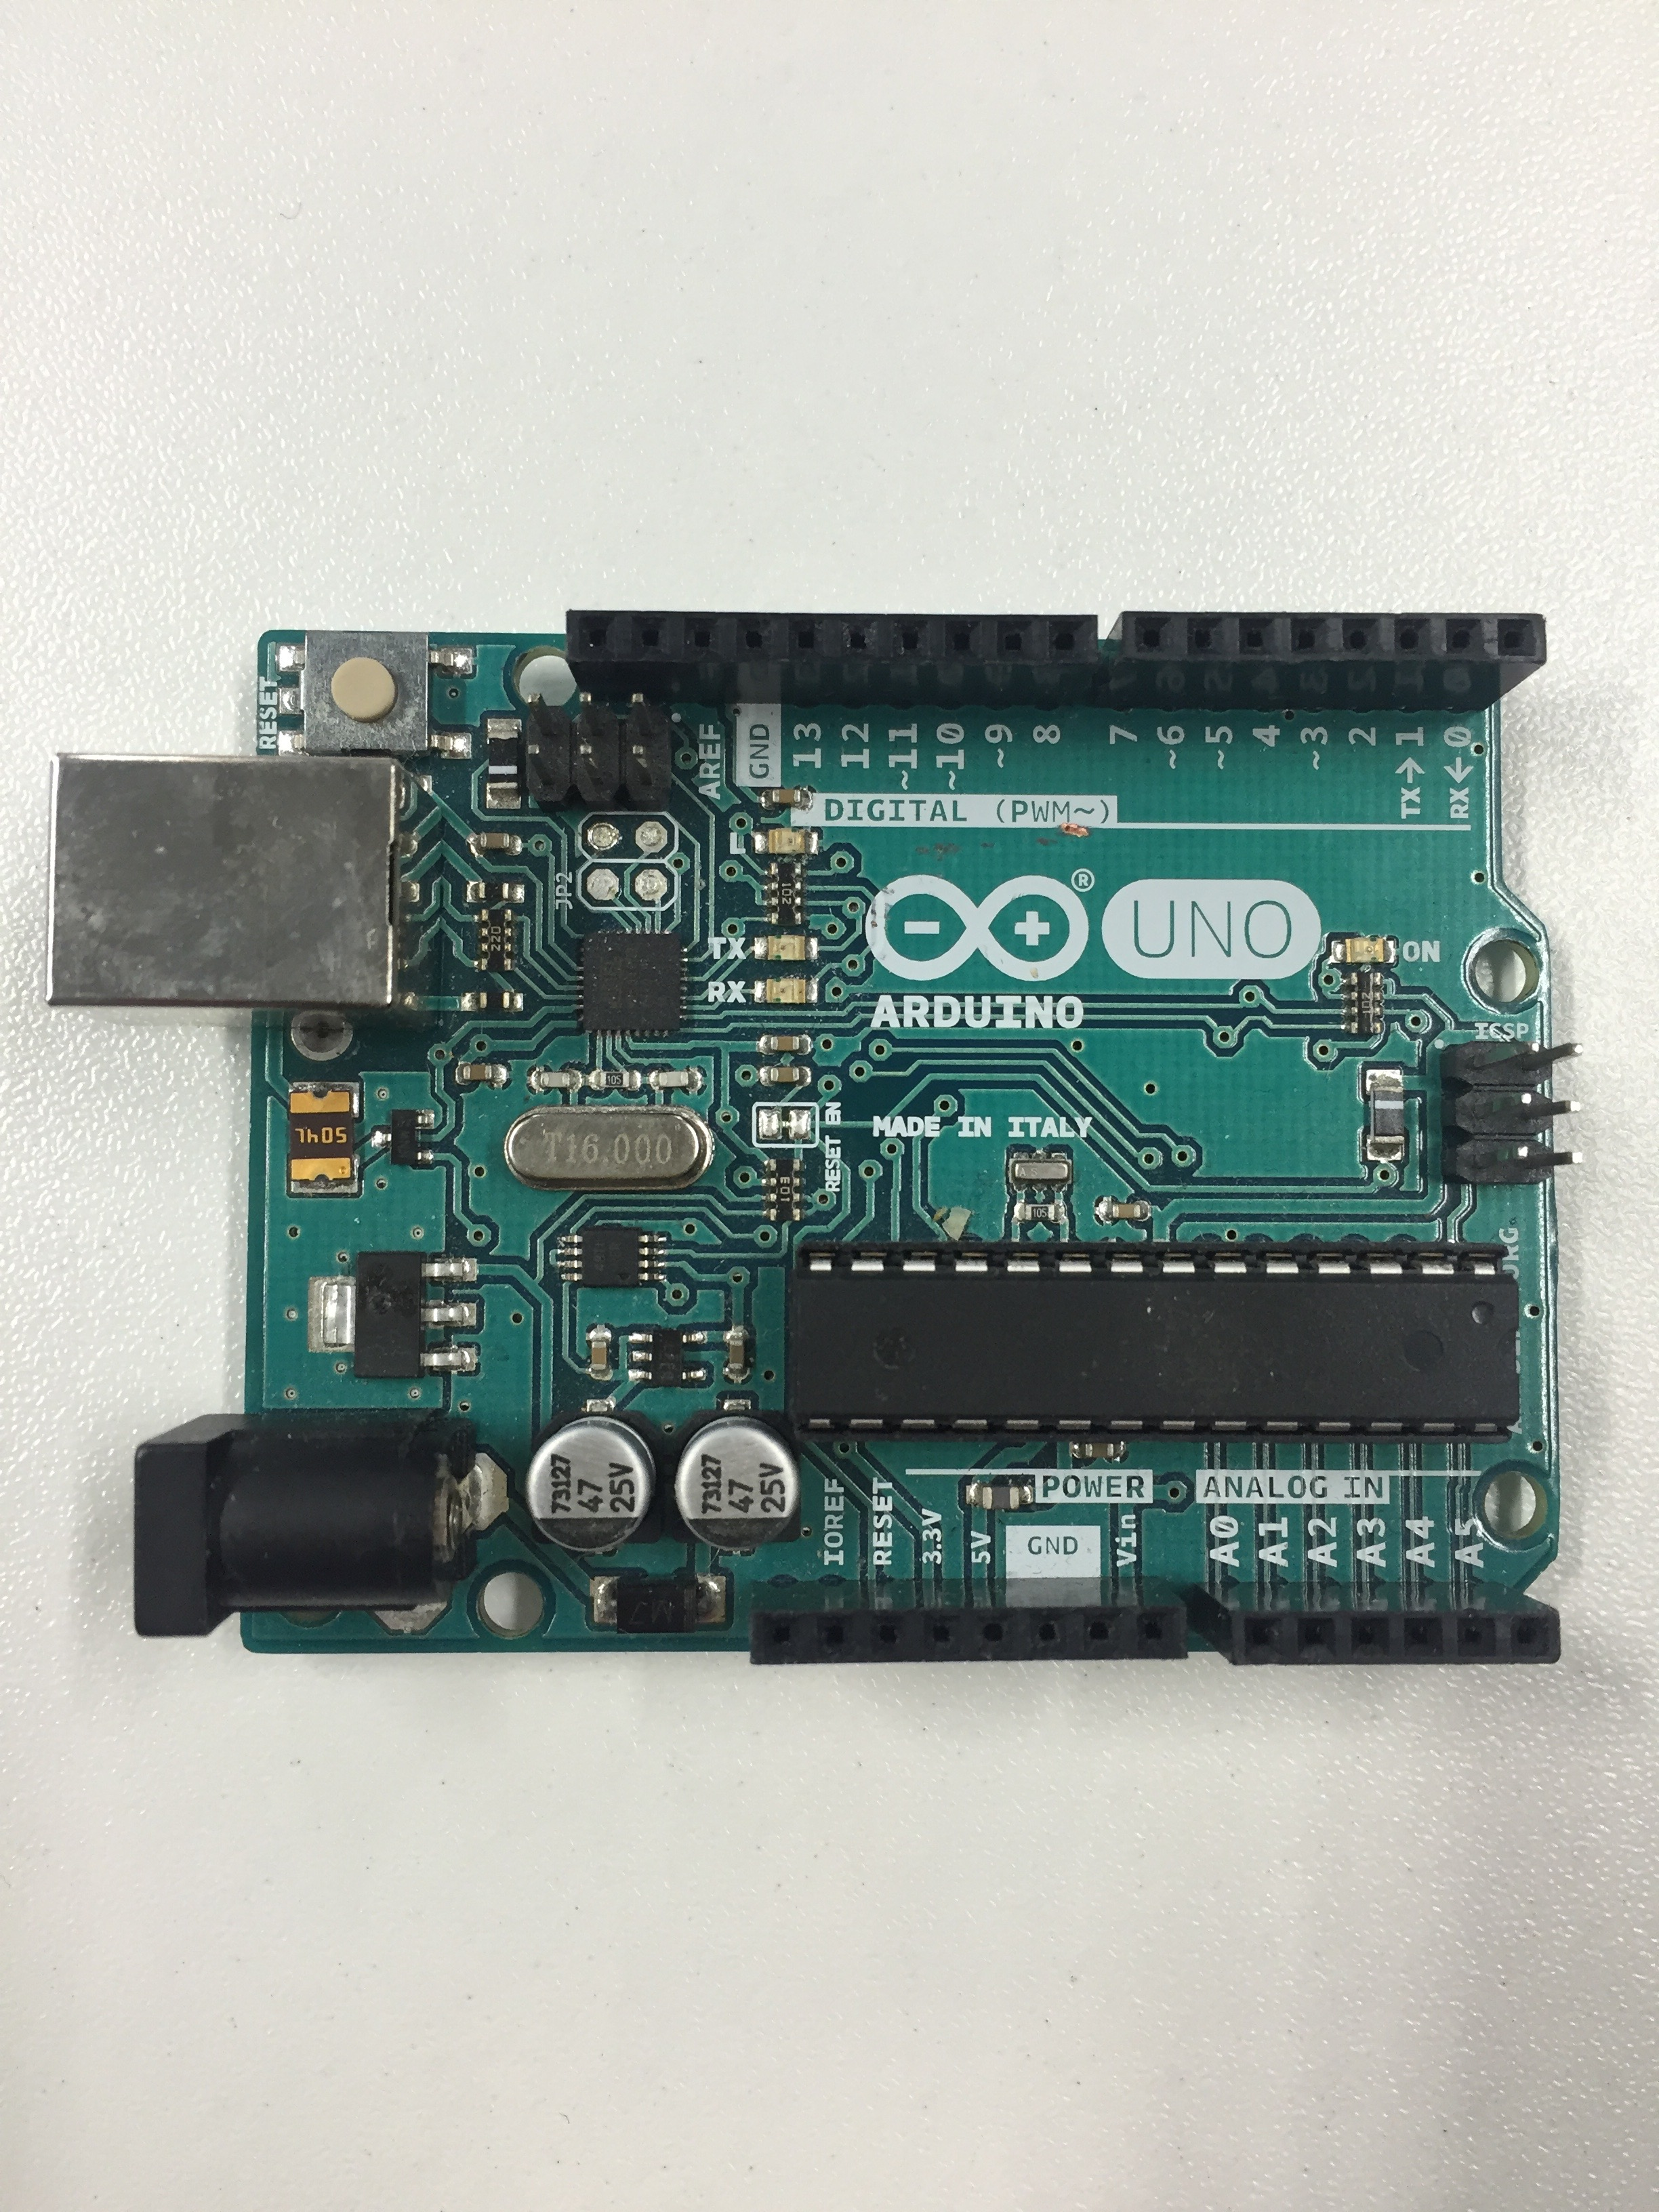
\includegraphics[trim={0 28cm 0 30cm}, clip, width=3in]{./media/microController.jpg}
\label{fig:MicroController}
\end{figure}
Pins: The top row are the digital pins (used with digitalRead(), digitalWrite and analogWrite)
In the bottom right, we have the analog pins (used with analogWrite).
Next to it, (bottom central), we have GND and 5V pins, to connect arduino to ground and provide
+5V power.
LED: LED 13, driven by pin 13.
Underneath are TX and RX LED's, indicating communication computer and Arduino.
To the right of the label, is the power pin (indicats if arduino receives power).
The microcontroller (an ATmega) is positioned underneath the label.
In the bottom left is the power connector where the batteries will be attached to.

\section{Building the thing}
The only actuators needed were two brushless DC motors.
\begin{figure}[h!]
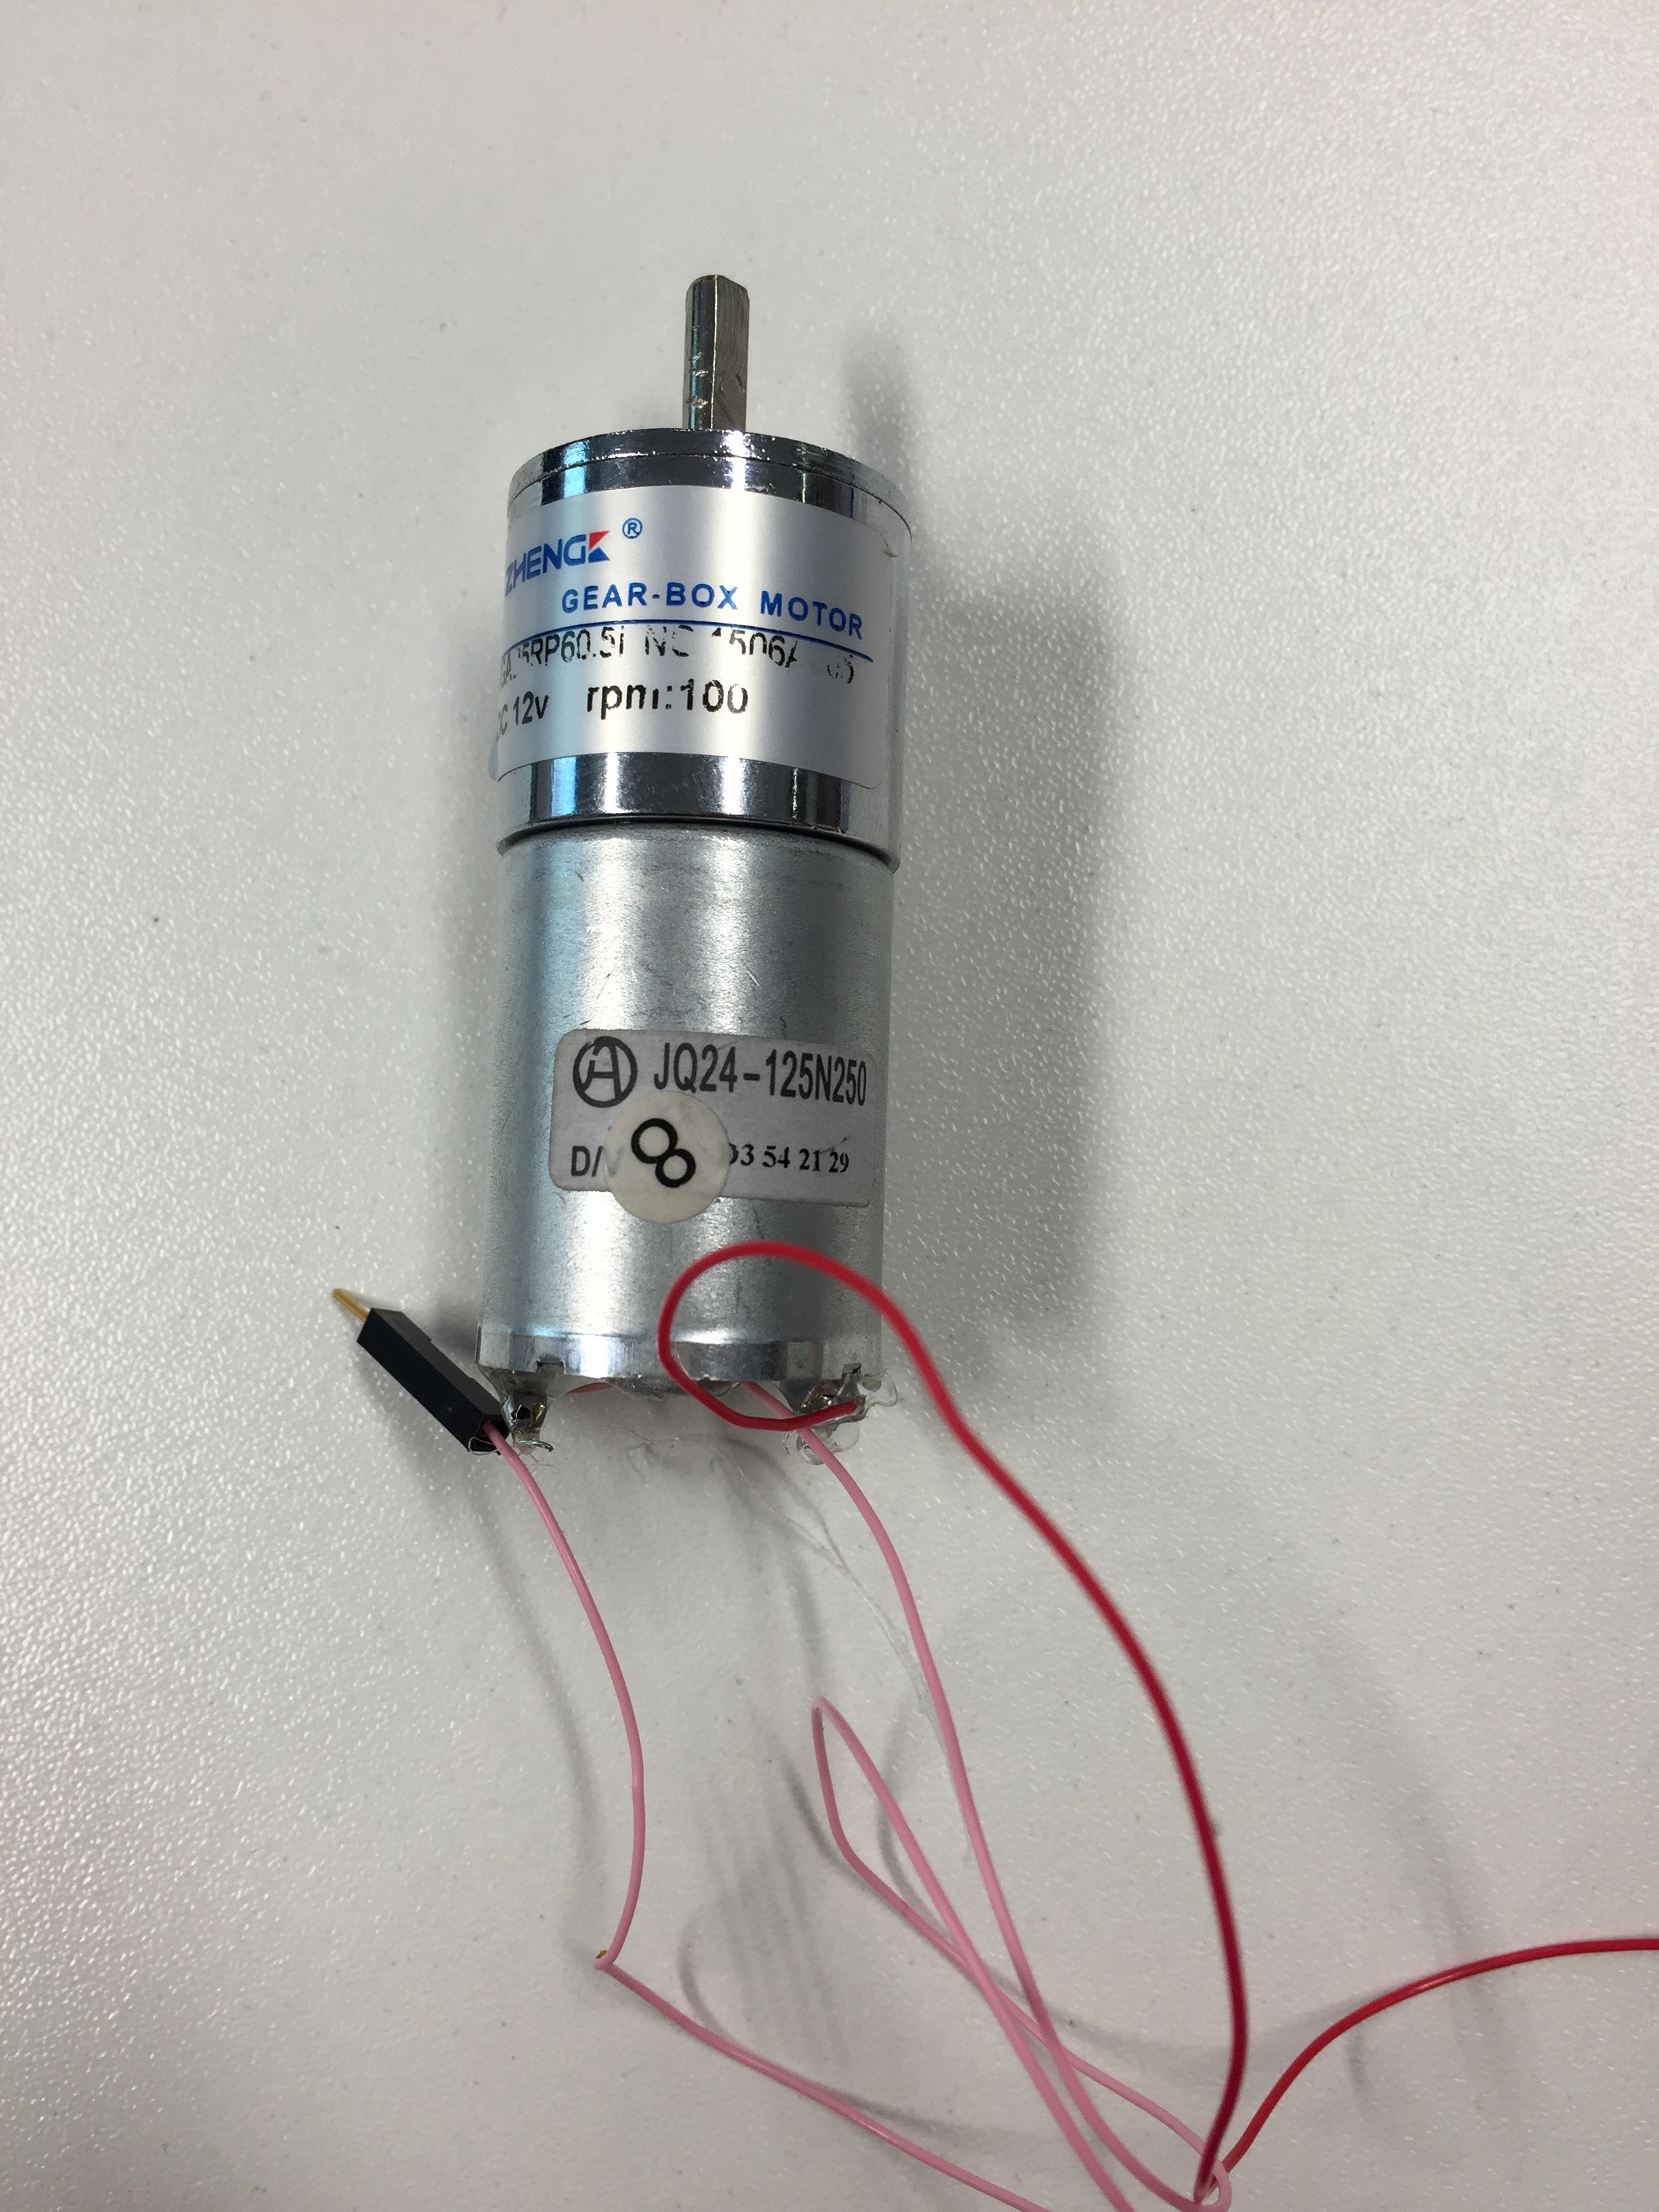
\includegraphics[trim={0cm 0cm 0cm 0cm}, clip, width=3in]{./media/motor.jpg}
\end{figure}
Each motor requires a current of 0.5 amps and a voltage of at least 6V.
However, the Arduino Uno is only capable to providing 0.4 amps and 5 volts.
Solution:
With a motor driver circuit and a switch that operates at the Arduino current/voltage level (on means 5V, of means 0V),  I control the necessary amps and volts to change directions of the rotation.
Motor Driver:
\begin{figure}[h!]
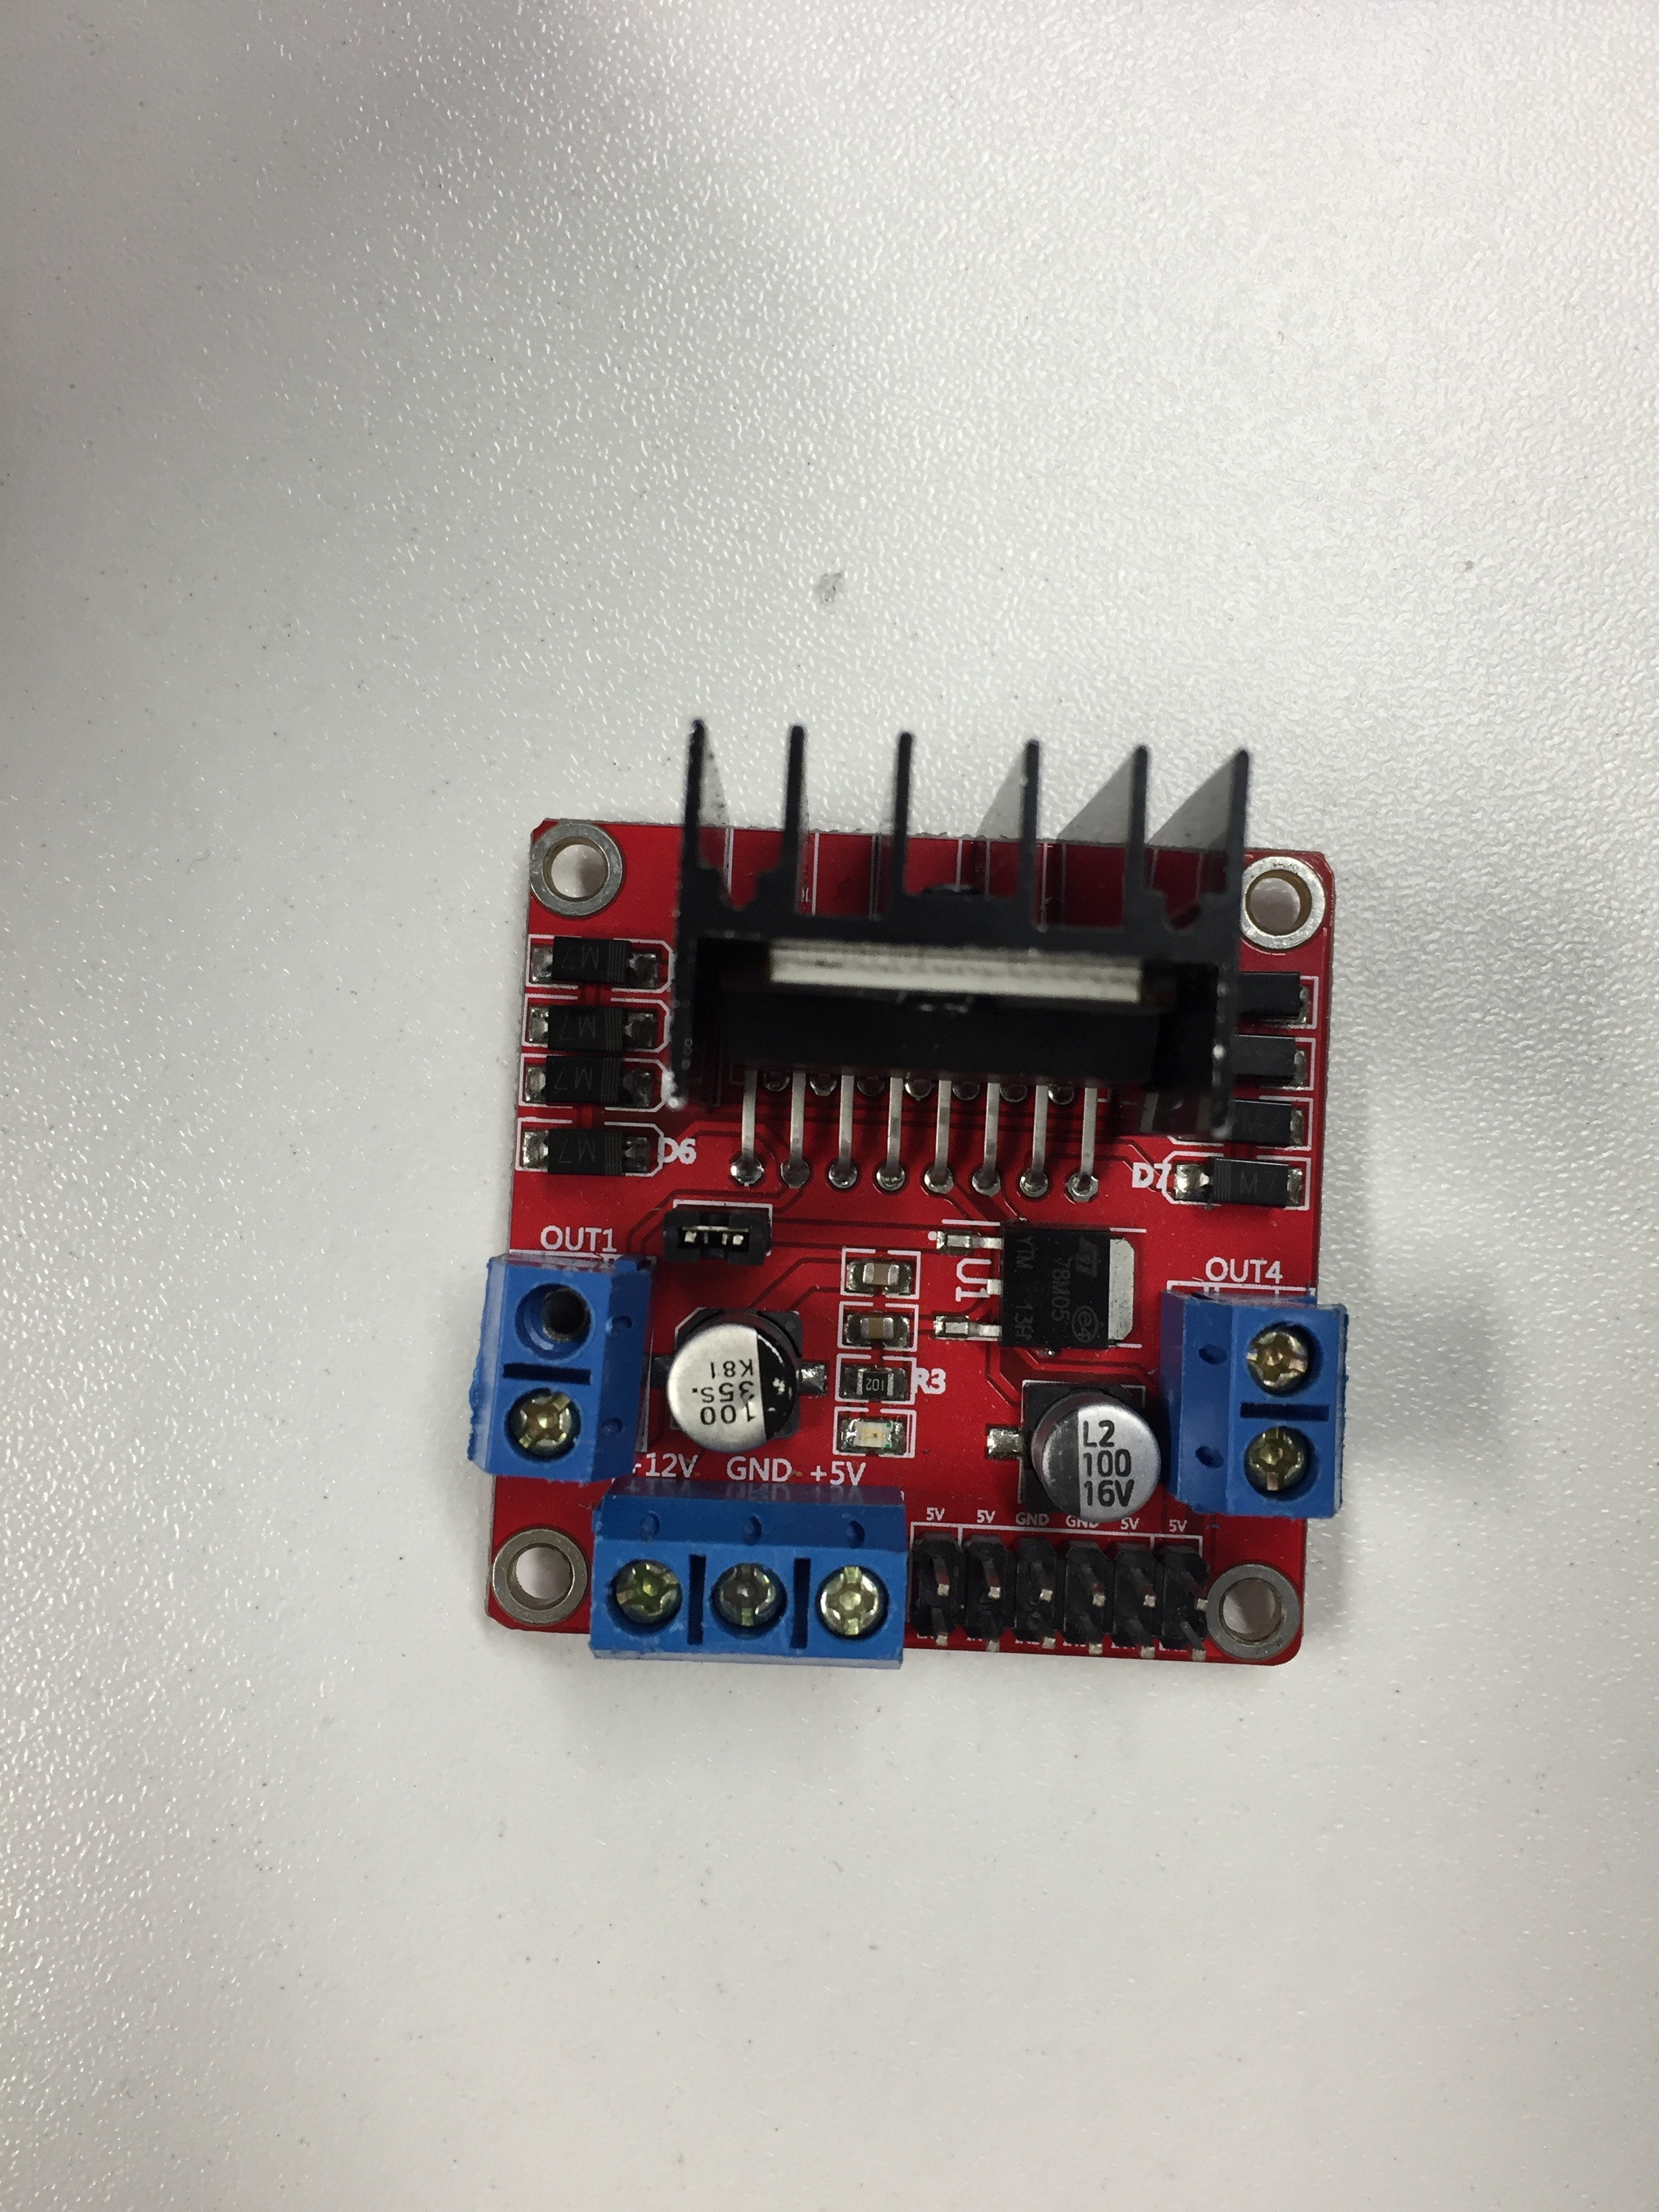
\includegraphics[trim={0cm 0cm 0cm 0cm}, clip, width=3in]{./media/motorDriver.jpg}
\end{figure}
\begin{figure}[h!]
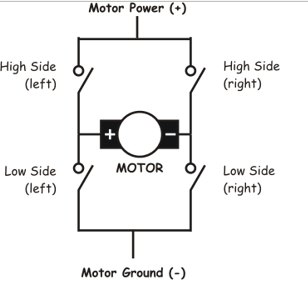
\includegraphics[trim={0cm 0.5cm 0cm 0.1cm}, clip, width=3in]{./media/hBridge.jpg}
source: http://www.mcmanis.com/chuck/robotics/tutorial/h-bridge/images/basic-bridge.gif
\end{figure}
Basically, the Driver is is arranged like an H-Bridge. When the switch is turned on (supplying 5V to Arduino), pin 2 will close, causing the motor to rotate clockwise. Similarly, when the switch is turned off (by supplying 0V), pin 3 will close and the motor will rotate in the opposite direction.

\section{Obstacle Avoidance}
The robot uses a sonar to detect obstacles. 
\begin{figure}[h!]
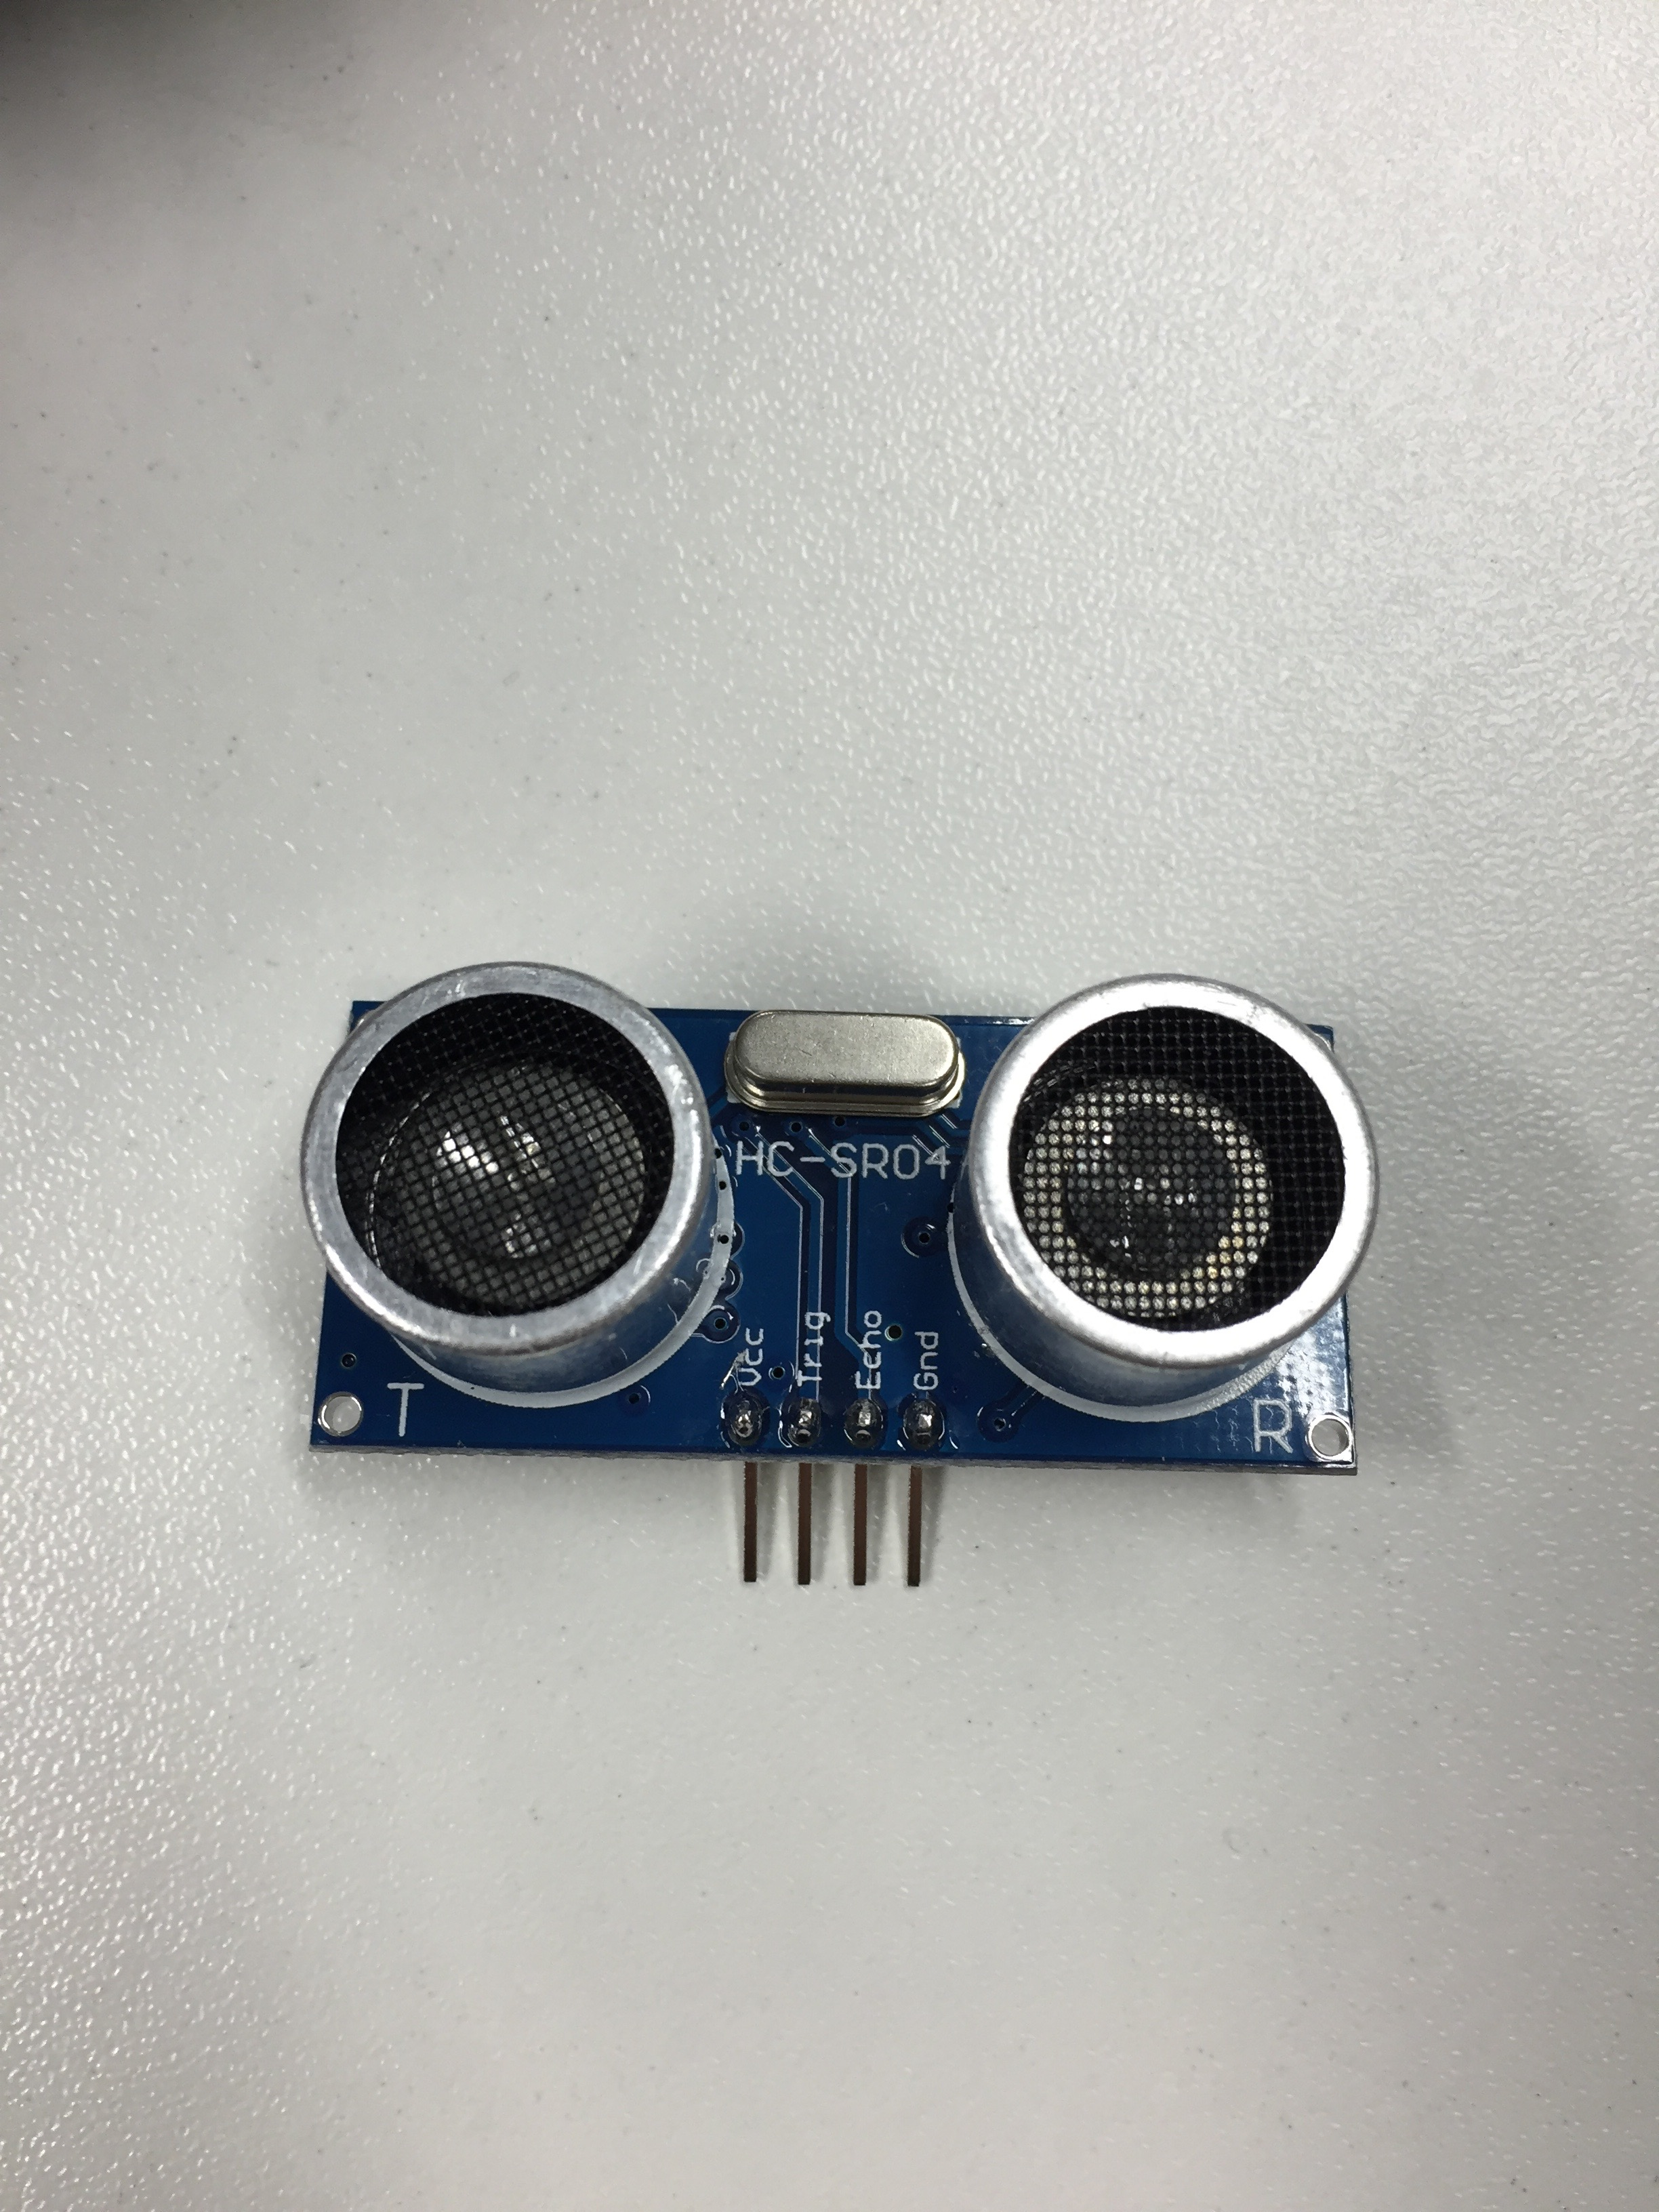
\includegraphics[trim={14cm 30cm 14cm 50cm}, clip, width=3in]{./media/Sonar.jpg}
\end{figure}
The sonar consists of a transmitter that sends out ultrasonic waves and a receiver which detects the reflection of these waves.
\begin{figure}[h!]
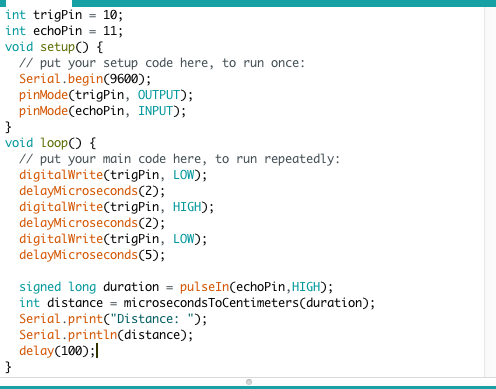
\includegraphics[trim={0cm 0cm 0cm 0cm}, clip, width=3in]{./media/sonarCode.jpg}
\end{figure}
The setup part is to "set up" the communication between sonar and Arduino.
In the Loop part, we tell the sonar to send out a low signal followed by a high signal followed by a low signal.
Using the pulseIn function we get the time it took (in microseconds) for the receiver to detect the reflection if the high signal.
Finally, using the (self-defined) "microsecondsToCentimeters" function, we get the distanceat which the wave has been reflected.
\begin{figure}[h!]
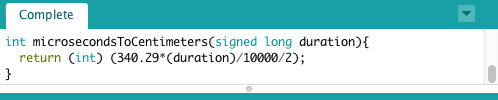
\includegraphics[trim={0cm 0cm 0cm 0cm}, clip, width=3in]{./media/sonarDistanceFunction.jpg}
\end{figure}
This next part of the code is somewhat arbitrary.
\begin{figure}[h!]
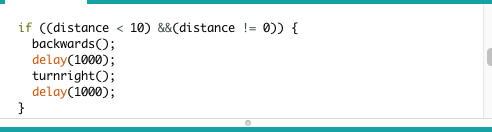
\includegraphics[trim={0cm 0cm 0cm 0cm}, clip, width=3in]{./media/obstacleAvoidance.jpg}
\end{figure}
It basically says: "when you get within 10cm of an object, go back a little and change direction".

\section{Light Follower}
/*Picture of LDR*/
To detect changes in Light intensity, I used two light dependent resistors (LDR's).
In simple terms:
Change in light intensity (arrow) change in resistance (arrow) change in voltage
The Arduino has a builtin analog-to-digital converter (ADC), with a 10 bit resolution.
This means at maximum light intensity, it will read the value 2pow(10)-1 (1023), and 0 when there is no light.
\begin{figure}[h!]
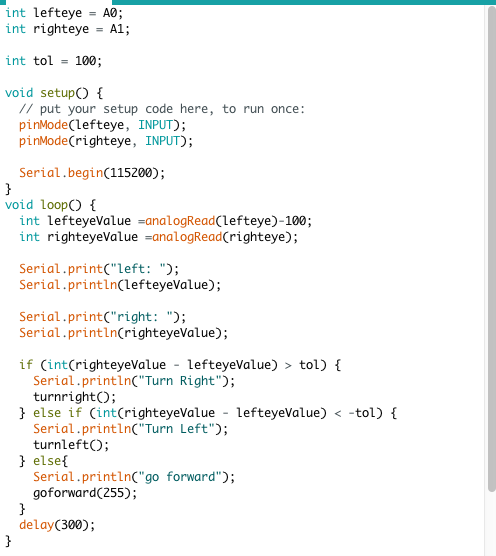
\includegraphics[trim={0cm 0cm 0cm 0cm}, clip, width=3in]{./media/lightFollower.jpg}
\end{figure}
Decreasing the light intensity, increases the resistance and according to Ohm's law, also the voltage.
Therefore the side that reads reads a lower value will be the brighter one.
A tolerance of 50 seemed to work fine in a dark room. In a brighter room, you'll have decrease the tolerance (unless you have a ridiculously strong flash light).
Unfortunately, this made the robot more susceptible to unrelated sources of light. 

\end{document}
